\autoref{fig:greedy.eks} er et eksempel på en grådig algoritme, som har forsøgt at finde den længst mulige simple vej i en graf.

\begin{figure}[H]
\centering
	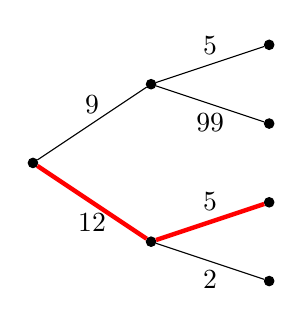
\begin{tikzpicture}

      \tikzset{enclosed/.style={draw, circle, inner sep=0pt, minimum size=.12cm, fill=black}}
% Vertices
      	\node[enclosed] (v1) at (0,2) {};
      	\node[enclosed] (v2) at (1.5,1) {};
    	\node[enclosed] (v3) at (1.5,3) {};
  	    \node[enclosed] (v4) at (3,0.5) {};
  	    \node[enclosed] (v5) at (3,1.5) {};
  	    \node[enclosed] (v6) at (3,3.5) {};
  	    \node[enclosed] (v7) at (3,2.5) {};    
%Edges
		\path (v1) edge[red, ultra thick] node[midway, below, black] {$12$} (v2);
		\path (v1) edge node[midway, above] {$9$} (v3);
		\path (v2) edge[red, ultra thick] node[midway, above, black] {$5$} (v5);
		\path (v2) edge node[midway, below] {$2$} (v4);
		\path (v3) edge node[midway, above] {$5$} (v6);
		\path (v3) edge node[midway, below] {$99$} (v7);


	\end{tikzpicture}
	\caption{Længste vej ifølge grådig algoritme.}
	\label{fig:greedy.eks}
\end{figure}

Vi kan se, at algoritmen har valgt de lokalt optimale valg, men den har ikke fundet den globalt optimale løsning. Det er tydeligt at se, at denne algoritme ikke er pålidelig nok til at løse sådanne problemer, da den ikke konsekvent finder den globalt optimale løsning. Der findes dog nogle grådige algoritmer, som er optimeret, så de altid finder den globalt optimale løsning, så længe grafen overholder specifikke krav. Dette ser vi i \autoref{kap:dijkstras}.

